\documentclass[14pt]{extarticle}

\usepackage{fontspec}
\setmainfont{Times New Roman}

% размер полей
\usepackage{geometry}
\geometry{a4paper, top=2cm, bottom=2cm, right=1.5cm, left=3cm}

 %debugging
%\usepackage{showframe}

% полуторный интервал
\usepackage{setspace}
\onehalfspacing

% абзацный отступ
\setlength{\parindent}{1.25cm}

% выравнивание текста по ширине
\sloppy

% списки
\usepackage{calc} % арифметические операции с величинами
\usepackage{enumitem}
\setlist{
    nosep,
    leftmargin=0pt,
    itemindent=\parindent + \labelwidth - \labelsep,
}

% подписи к рисункам и таблицам
\usepackage{caption}
\renewcommand{\figurename}{Рисунок}
\renewcommand{\tablename}{Таблица}
\DeclareCaptionFormat{custom}
{
    \textit{#1#2#3}
}
\DeclareCaptionLabelSeparator{custom}{. }
\captionsetup{
    % хз какой это размер - 12 или нет, но выглядит меньше 14
    font=small,
    format=custom,
    labelsep=custom,
}

% картинки
\usepackage{graphicx}

% колонтитулы
\usepackage{fancyhdr}

% картинки и таблицы находятся именно в том месте текста где помещены (атрибут H)
\usepackage{float}

% таблицы
\usepackage{tabularray}

\graphicspath{ {2.2.1/models/} }
\begin{document}
\pagestyle{fancy}
\fancyhead{}
% disable header
\renewcommand{\headrulewidth}{0pt}
\fancyfoot[L]{Дубровских гр 221-361}
\fancyfoot[C]{ЛР 2.2.1}
\fancyfoot[R]{Продажа автотранспорта}
\singlespacing

\newpage
\begin{center}
    Министерство науки и высшего образования Российской Федерации
    Федеральное государственное автономное образовательное учреждение

    высшего образования

    \guillemotleft МОСКОВСКИЙ ПОЛИТЕХНИЧЕСКИЙ УНИВЕРСИТЕТ\guillemotright

    (МОСКОВСКИЙ ПОЛИТЕХ)
\end{center}
\noindent
\bigbreak
\bigbreak
\bigbreak
\bigbreak
\begin{center}
    ЛАБОРАТОРНАЯ РАБОТА 2.2.1

    По курсу Проектирования пользовательских интерфейсов в веб
    \textbf{Разработка пользовательских сценариев. Составление блок-схем типичного сценария

}
    \bigbreak
    \bigbreak
    \bigbreak
    \bigbreak
    ТЕМА

    \guillemotleft\textbf{САЙТ ДЛЯ ПРОДАЖИ И ПОИСКА АВТОМОБИЛЕЙ}\guillemotright
\end{center}
\noindent
\bigbreak
\bigbreak
\bigbreak
\bigbreak
\bigbreak
\bigbreak
\bigbreak
\bigbreak
\bigbreak
\bigbreak
\hfill Выполнил

\hfill Дубровских Никита Евгеньевич

\hfill Группа 221-361
\bigbreak
\bigbreak
\bigbreak
\hfill Проверил

\hfill Натур ВВ
\vfill
\begin{center}
    Москва, 2024
\end{center}
\newpage
\onehalfspacing


\begin{center}
    \textbf{Лабораторная работа 2.2.1}

    \textbf{РАЗРАБОТКА ПОЛЬЗОВАТЕЛЬСКИХ СЦЕНАРИЕВ. СОСТАВЛЕНИЕ БЛОК-СХЕМ ТИПИЧНОГО СЦЕНАРИЯ}
\end{center}

\textbf{Цель работы:} придумать все возможные варианты взаимодействия пользователей и интерфейса.
\bigskip

\textbf{Задачи:}

\begin{enumerate}
    \item В виде блок-схем или в виде списка разработать возможные сценарии использования проектируемого интерфейса.
    \item Проанализировать полученные результаты и оптимизировать временные затраты (свести к минимуму количество шагов пользователя для достижения его целей).

\end{enumerate}
\bigskip

\textbf{Основные термины}

\begin{itemize}
    \item Пользовательские сценарии - наглядное схематическое представление того, как пользователь решает свою задачу с помощью сайта или приложения.
    \item Блок-схемы - графическое представление сценариев использования, показывающее последовательность действий пользователя.
    \item Сценарий использования (Use case) - описание поведения системы при взаимодействии с внешней средой.
    \item Пользовательские маршруты (User flows) - последовательность шагов, которые пользователь проходит для достижения своей цели на сайте или в приложении.
    \item Диаграмма потоков задач (Task flows) - визуальное представление шагов, необходимых для выполнения задачи пользователем.
    \item Оптимизация временных затрат - процесс минимизации количества шагов пользователя для достижения его целей.
    \item Варианты использования - список шагов, которые может пройти пользователь для достижения своей цели.
\end{itemize}
\bigskip

\textbf{Сценарии использования}

Сценарий 1: Поиск автомобиля

\begin{enumerate}
    \item пользователь заходит на сайт;
    \item пользователь видит главную страницу с поисковой строкой;
    \item пользователь вводит марку и модель автомобиля в поисковую строку;
    \item пользователь нажимает кнопку "Поиск";
    \item система отображает список автомобилей, соответствующих запросу;
    \item пользователь просматривает список и выбирает интересующий автомобиль;
    \item пользователь переходит на страницу с подробной информацией об автомобиле;
    \item пользователь может связаться с продавцом или сохранить объявление.
\end{enumerate}
\bigskip

Сценарий 2: Размещение объявления о продаже автомобиля

\begin{enumerate}
    \item пользователь заходит на сайт;
    \item пользователь нажимает кнопку ”Подать объявление”;
    \item пользователь заполняет форму с информацией о автомобилe (марка, модель, год выпуска, цена, описание, фотографии);
    \item пользователь нажимает кнопку ”Опубликовать”;
    \item система подтверждает успешное размещение объявления;
    \item пользователь получает уведомление о размещении объявления.
\end{enumerate}
\bigskip

Сценарий 3: Фильтрация результатов поиска

\begin{enumerate}
    \item пользователь заходит на сайт;
    \item пользователь вводит запрос в поисковую строку;
    \item система отображает список автомобилей;
    \item пользователь использует фильтры (цена, год выпуска, пробег, тип кузова) для уточнения поиска;
    \item система обновляет список автомобилей в соответствии с выбранными фильтрами;
    \item пользователь выбирает интересующий автомобиль и переходит на страницу с подробной информацией.
\end{enumerate}
\bigskip

Сценарий 4: Сравнение автомобилей

\begin{enumerate}
    \item пользователь заходит на сайт;
    \item пользователь вводит запрос в поисковую строку и получается список автомобилей;
    \item пользователь выбирает несколько автомобилей для сравнения (отмечает галочками);
    \item пользователь нажимает кнопку ”Сравнить”;
    \item система отображает таблицу сравнения выбранных автомобилей по ключевым характеристика;
    \item пользователь анализирует сравнение и выбирает интересующий автомобиль для дальнейшего изучения.
\end{enumerate}
\bigskip

\textbf{Анализ полученных результатов и оптимизация временных затрат}

Исходя из составленных вариантов использования можно сформировать следующие оптимизации временных затрат:

\begin{itemize}
    \item Упрощение навигации: главная страница содержит четкие и понятные ссылки на основные функции (поиск, размещение объявления, фильтры). Это поможет пользователю быстрее находить нужные разделы.
    \item Автозаполнение: внедрить функцию автозаполнения в поисковой строке, что может сократить время, необходимое для ввода данных, и уменьшить количество ошибок.
    \item Сохранение поиска: позволить пользователям сохранять свои поисковые запросы и фильтры, чтобы они могли быстро возвращаться к ним в будущем.
    \item Упрощение формы размещения объявления: форма для размещения объявления максимально проста и интуитивно понятна. Использовать подсказки и примеры, чтобы помочь пользователям заполнить форму быстрее.
    \item Оптимизация загрузки страниц: за счёт сжатия изображений, использование технологий кэширования страницы загружаются быстро, чтобы пользователи не теряли время на ожидание.
    \item Мобильная версия: удобный интерфейс для мобильных устройств, так как многие пользователи могут заходить на сайт с телефонов.
\end{itemize}
\bigskip

\textbf{Блок-схемы с минимальным количеством шагов}
\bigskip

\noindent
\begin{minipage}{\linewidth}
    \centering
    \fbox{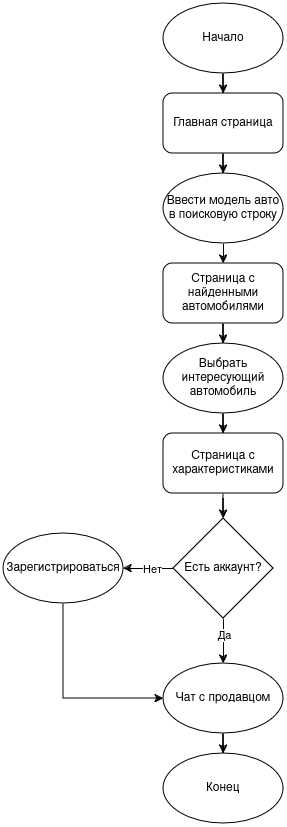
\includegraphics[scale=0.5]{ppi_221_scenario1.drawio}}
    \captionof{figure}{Диаграмма \guillemotleft Поиск автомобиля\guillemotright}
\end{minipage}
\bigskip

\noindent
\begin{minipage}{\linewidth}
    \centering
    \fbox{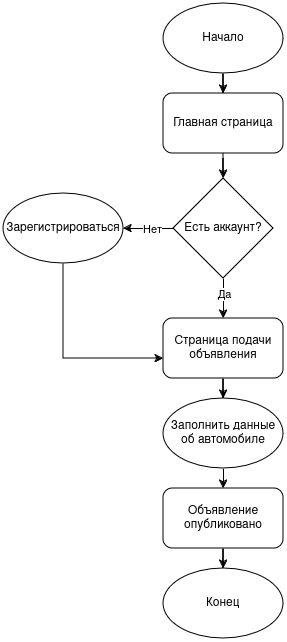
\includegraphics[scale=0.5]{ppi_221_scenario2.drawio}}
    \captionof{figure}{Диаграмма \guillemotleft Публикация объявления\guillemotright}
\end{minipage}
\bigskip

\noindent
\begin{minipage}{\linewidth}
    \centering
    \fbox{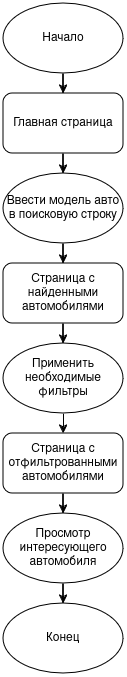
\includegraphics[scale=0.5]{ppi_221_scenario3.drawio}}
    \captionof{figure}{Диаграмма \guillemotleft Фильтрация по параметрам\guillemotright}
\end{minipage}
\bigskip

\noindent
\begin{minipage}{\linewidth}
    \centering
    \fbox{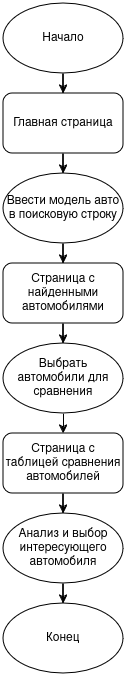
\includegraphics[scale=0.5]{ppi_221_scenario4.drawio}}
    \captionof{figure}{Диаграмма \guillemotleft Сравнение характеристик\guillemotright}
\end{minipage}
\bigskip

Определение минимальных шагов пользователя для достижения цели позволит создать линейный, интуитивно понятный интерфейс, без лишних кликов и действий. Каждый элемент интерфейса будет давать четкое представление о его функции, а ключевые элементы можно выделить цветом, размером, и расположением, что бы пользователь сразу понимал где искать нужное действие.

\textbf{Заключение}

Оптимизация пользовательских сценариев и минимизация шагов, необходимых для достижения целей, помогут улучшить пользовательский опыт и увеличить количество успешных взаимодействий на сайте.
\bigskip

\textbf{Контрольные вопросы и ответы}

\begin{enumerate}
    \item Что такое пользовательские сценарии и зачем они нужны?

    Пользовательские сценарии — это описания того, как пользователи взаимодействуют с продуктом (сайтом или приложением) для достижения своих целей. Они помогают понять потребности и поведение пользователей, а также выявить возможные проблемы в интерфейсе. Сценарии необходимы для проектирования удобных и эффективных интерфейсов, так как они позволяют разработчикам и дизайнерам сосредоточиться на реальных задачах пользователей.
    \item Что такое пользовательские маршруты (user flows) и зачем они нужны?

    Пользовательские маршруты (user flows) — это визуальные представления последовательности шагов, которые пользователь проходит для выполнения конкретной задачи в приложении или на сайте. Они помогают понять, как пользователи перемещаются по интерфейсу, какие действия выполняют и какие решения принимают. Пользовательские маршруты необходимы для оптимизации навигации и улучшения пользовательского опыта, позволяя выявить узкие места и улучшить взаимодействие.
    \item Что такое «диаграмма потоков задач» (Task flows)? На каком этапе и как ее строят?

    Диаграмма потоков задач (Task flows) — это графическое представление шагов, необходимых для выполнения конкретной задачи пользователем. Она строится на этапе проектирования, когда уже собраны данные о потребностях пользователей и определены основные сценарии использования. Для создания диаграммы потоков задач используются блоки, представляющие действия пользователя, и стрелки, показывающие направление потока. Это помогает визуализировать процесс и выявить возможные улучшения.
    \item Расскажите про основные элементы диаграмм потоков задач.

    Основные элементы диаграмм потоков задач включают:
    блоки действий - представляют собой шаги, которые пользователь должен выполнить (например, "Нажать кнопку", "Заполнить форму"),
    стрелки - показывают направление потока и последовательность действий,
    решения - точки, где пользователь может выбрать один из нескольких вариантов (например, "Да/Нет"),
    начало и конец - обозначают стартовую и конечную точки процесса,
    подпроцессы - могут быть использованы для обозначения более сложных действий, которые могут быть разбиты на отдельные шаги.
\end{enumerate}

\end{document}
